\documentclass{cernatsnote}
\usepackage[colorinlistoftodos]{todonotes}
\usepackage{placeins}
\usepackage{listings}
\usepackage{tabularx}
\usepackage{siunitx}


\usepackage{color} % for setting colors
% set the default code style
\lstset{
    language=Python,
    backgroundcolor=\color{black!5}, 
    basicstyle=\ttfamily\small,
    keywordstyle=\color{blue},
    stringstyle=\color{red},
    commentstyle=\color{green},
    morecomment=[l][\color{magenta}]{\#},
    frame=single, % adds a frame around the code
    breaklines=true, % sets automatic line breaking
    breakatwhitespace=true, % sets if automatic breaks should only happen at whitespace
    tabsize=4, % sets default tabsize to 4 spaces
    captionpos=b, % sets the caption-position to bottom
    escapeinside={\%*}{*)}, % if you want to add LaTeX within your code
    morekeywords={*,...} % if you want to add more keywords to the set
}


\title{Multiple Couloumb Scattering simulation for optics design}
\author{
	Eliott Philippe Johnson \; \\		
	CERN, CH-1211 Geneva, Switzerland
}
\email{eliott.philippe.johnson@cern.ch}
\date{\today}

\begin{document}
\maketitle

\begin{abstract}
This document presents the integration of the Multiple Coulomb Scattering process in MAD-X which is useful for the optics design at CERN. This integration is compared to other simulations and to measurement. 
\end{abstract}
\\ \\ \\ 

\begingroup
\color{black}
\tableofcontents
\endgroup

\pagebreak

\section{Introduction}
In the context of the ion irradiation activity in the East Area (CHIMERA and HEARTS), knowledge of the beam size on the device under test (DUT) is of particular importance. One of the challenges in modelling the optics of the line is that the beam crosses multiple air regions which increase the beam size. The air scattering effects need to be studied and included.

\section{Objective}
% Detail the main goal of your project.

The objective is to be able to match optics in MAD-X or similar tools with a model of the line that account for the air regions and the subsequent air scattering and emittance blow up. To achieve this, the simulation must be computationally efficient to allow rapid iterations within an optimization loop. The present works shows the implementation and benchmark to other simulation tools of multiple coulomb scattering in MAD-X and the comparison to measurements.

\section{Methodology}
% Describe the approach, algorithms, and models you used in your implementation.

The approach chosen to simulate multiple coulomb scattering was to use an analytical model where the formalism described by A.-S Müller \cite{muller_description_2001} is followed. The root mean square of the scattering angle, $\theta_{rms}$, is calculated using the momentum, $p$ in \SI{}{\mega\electronvolt\per\text{c}}, of the beam, the relativistic beta factor, $\beta_{p}$, the charge of the particle, $q_{p}$, the distance, $L$ in \SI{}{m}, of material travelled through and the radiation length $L_{rad}$ in \SI{}{m}.

$$\theta_{rms} = \frac{13.6 MeV/c}{p\beta_{p}}q_{p} \sqrt{ \frac{L}{L_{rad}} }$$

the twiss parameters after beam matter interaction are calculated using:

$$\alpha = \frac{\varepsilon_0 \alpha_0 - \frac{L}{2}\langle\theta^2\rangle} {\varepsilon_0 + \Delta\varepsilon}$$
$$\beta = \frac{\varepsilon_0 \beta_0 + \frac{L^2}{3}\langle\theta^2\rangle}{\varepsilon_0 + \Delta\varepsilon}$$
$$\gamma = \frac{\varepsilon_0 \gamma_0 + \langle\theta^2\rangle}{\varepsilon_0 + \Delta\varepsilon}$$

where $\alpha_{0}, \beta_{0}, \gamma_{0}$ are the twiss parameter in both planes at the start of the interaction. The beam emittance growth is calculated using: 

$$\Delta\epsilon = \frac{1}{2} \langle \theta^2 \rangle \left[ \beta_0 + L\alpha_0 + \frac{L^2}{3} \gamma_0 \right]$$

where $\Delta\epsilon$ is the change in emittance after beam-matter interactions. With $L_{rad}=\SI{301}{m}$ for air at standard pressure.

\section{Implementation}
% Discuss how you integrated the module into MAD-X, including any code snippets or algorithms.

The MAD-X implementation was chosen so that air region can be easily added to existing lines (sequences). As such, air regions can be added using the add\_air\_region function which takes as argument the start and stop location of the air region is s-coordinate and the granularity of the air region division.
\\
\begin{lstlisting}[language=Python, caption=Python example]
simple_seq: SEQUENCE, refer = exit, l = 100;
QF1 : QF1, AT=2;
QD2 : QD2, AT=5;
QF3 : QF3, AT=8;
QD4 : QD4, AT=11;
END : MARKER, AT=100;
ENDSEQUENCE;

sequence = "simple_seq"
add_air_region(madx, "1", sequence, 20, 30, 1)
\end{lstlisting}

An \href{https://gitlab.cern.ch/abt-optics-and-code-repository/simulation-codes/pybt/-/blob/master/pybt/examples/example_air_scattering.ipynb?ref_type=heads}{example of air scattering} is available in the \href{https://gitlab.cern.ch/abt-optics-and-code-repository/simulation-codes/pybt/}{PyBT repository}. This example shows a simple line of a $\SI{100}{m}$ with four quadrupoles to which three air regions are added. Each air region is separated in subdivisions of different lengths as shown in Fig. \ref{fig:example_air_scattering}.

\begin{figure}[!htb]
\centering
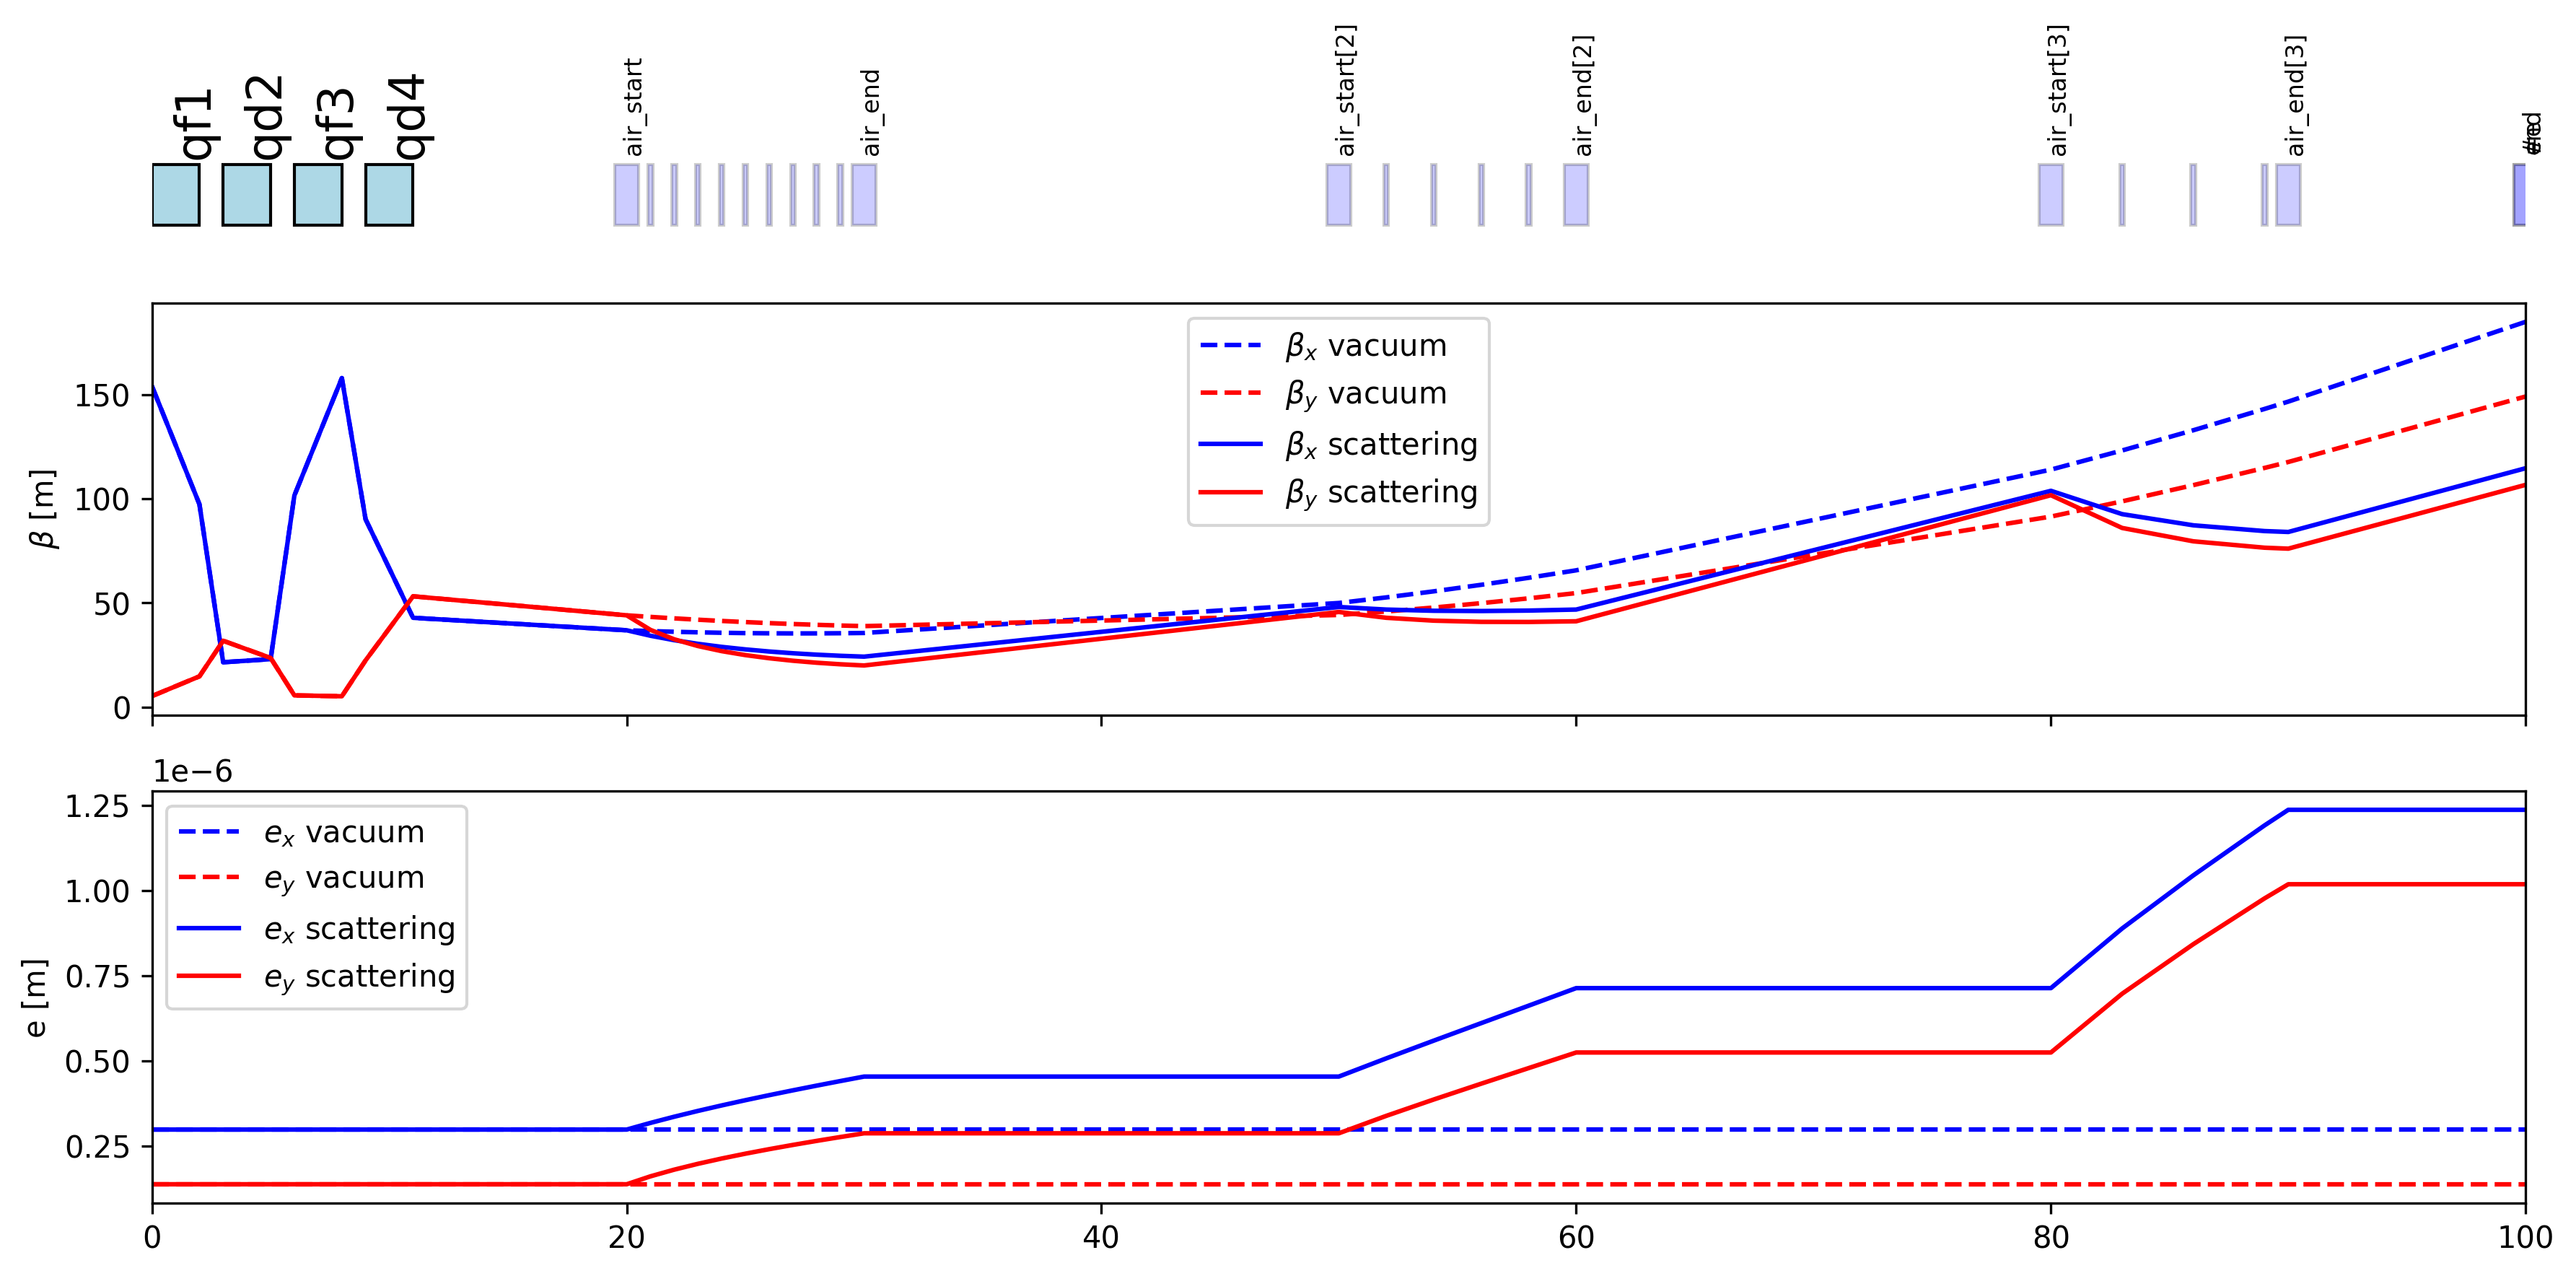
\includegraphics[width=1.0\textwidth]{images/example_air_scattering.png}
\caption{Example of air scattering.}
\label{fig:example_air_scattering}
\end{figure}

The script's logic begins by adding air regions and placing inner markers, which delineate computation steps, within the transfer line. Initial Twiss parameters ($\alpha, \beta, \gamma, \varepsilon$) are inputted, leading to the calculation of an initial Twiss solution. The script then identifies the first air region marker and uses the twiss parameters at the first inner marker (i.e. the first step) and computes the new twiss parameters with the equations presented above. This updates $[\alpha,\beta,\gamma,\varepsilon] \rightarrow [\alpha^{'},\beta^{'},\gamma^{'},\varepsilon^{'}]$ at the inner marker. Following this, a smaller sequence is extracted which starts from the first inner marker to the end of the line. A new beam is created with the $[\alpha^{'},\beta^{'},\gamma^{'},\varepsilon^{'}]$ and a twiss is calculated. This loops through all inner marker and for each air region. Finally, the twiss\_scattered dataframe is produced by assembling all the twiss created and stitching them into a coherent twiss. Fig. \ref{fig:diagram_air_scattering} describes the script's logic in a diagram format.

\begin{figure}[!htb]
\centering
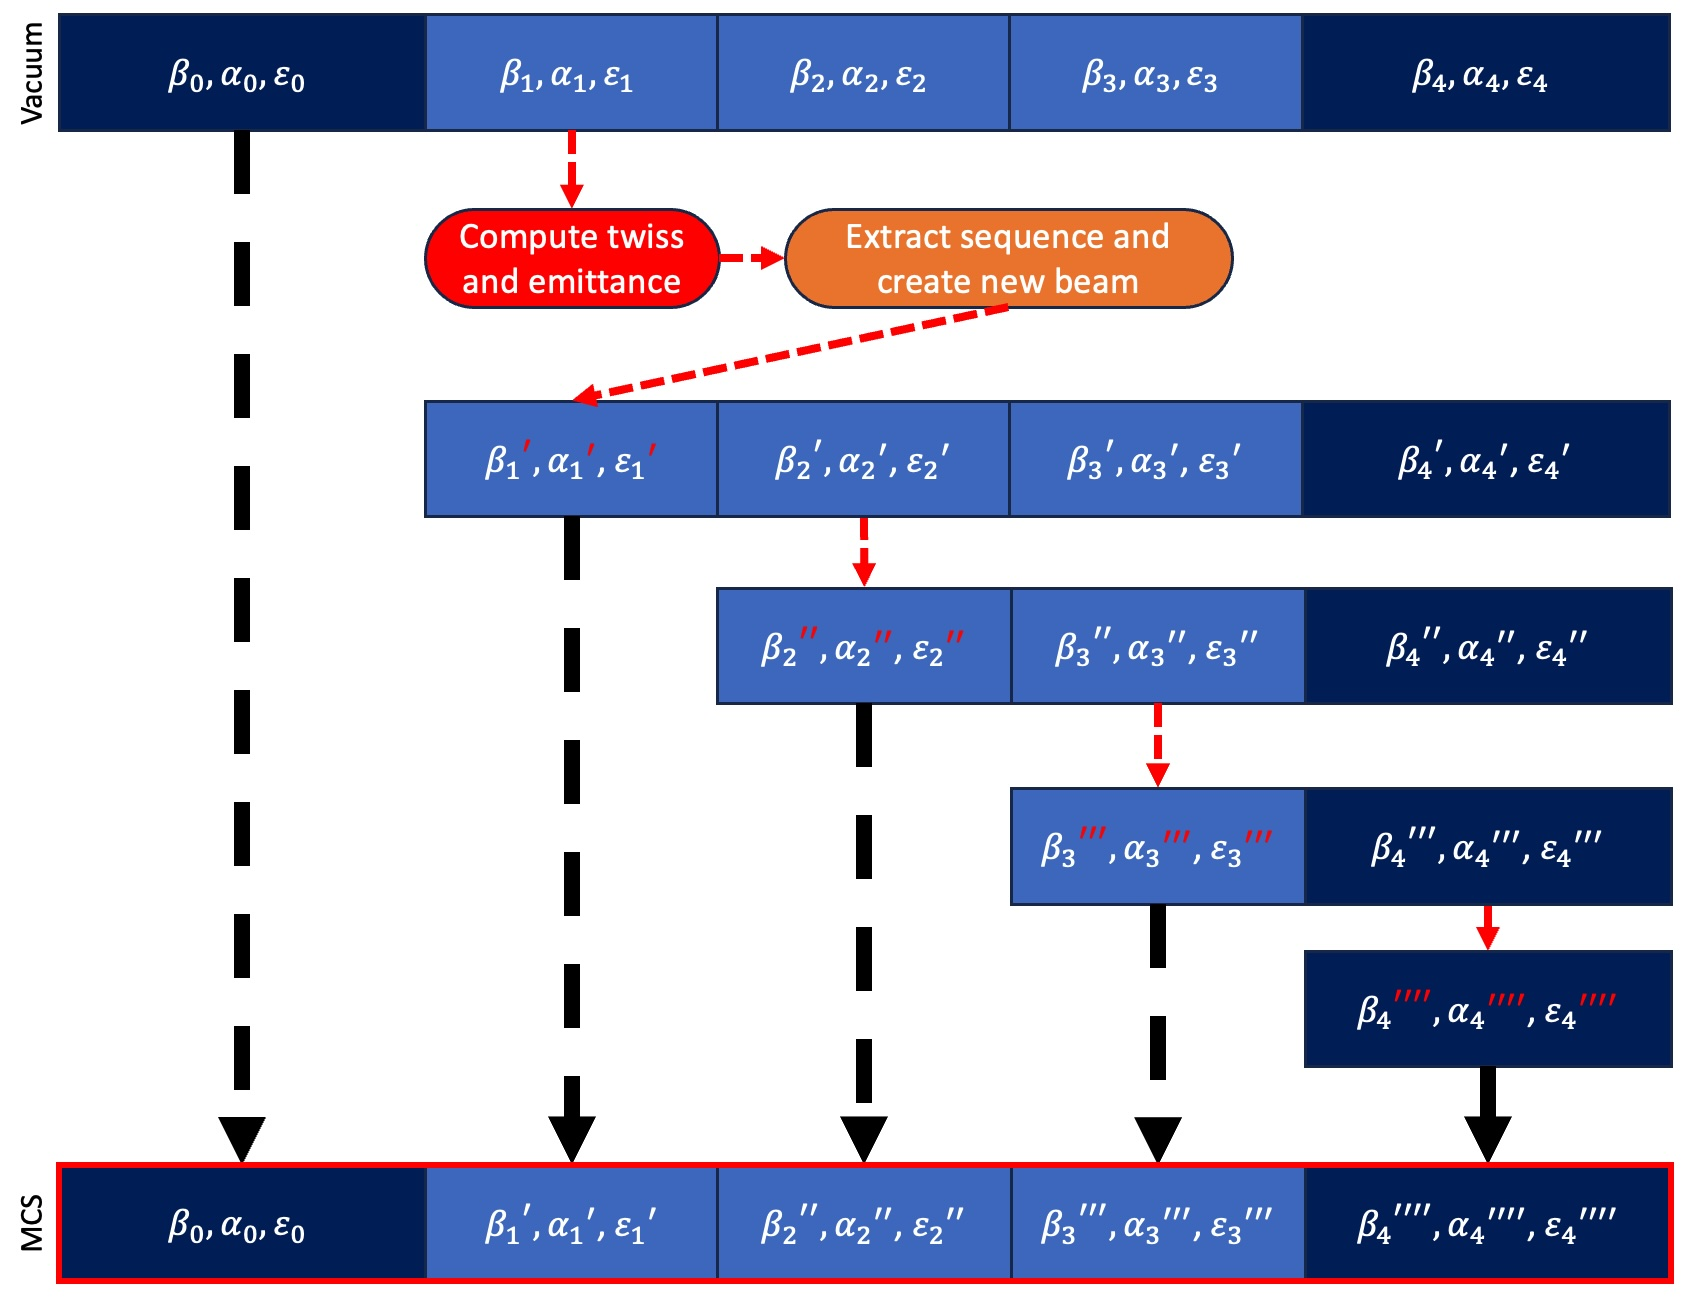
\includegraphics[width=0.7\textwidth]{images/diagram_air_scattering.jpg}
\caption{Diagram of air scattering.}
\label{fig:diagram_air_scattering}
\end{figure}

The code was designed so that the user can easily insert multiple air regions of different lengths. This is in part due to the fact that the F61 and T08 line in the East Area have numerous air region and that studies with and without certain part of the line in and out of vacuum could be studied.

\section{Results}
% Present your findings, including any data analysis or visualizations.

Figure \ref{fig:comparison_sim} shows the differences between three simulation tools (MAD-X, Xsuite and FLUKA) for multiple coulomb scattering. The Xsuite simulation uses the EverestBlock and an example can be found at the following link: \href{https://github.com/xsuite/xcoll/blob/main/examples/transfer_line_with_air.py}{transfer\_line\_with\_air.py} \cite{iadarola_xsuite_2023}. FLUKA simulations were provided by A. Waets \cite{ahdida_new_2022-1, battistoni_overview_2015}. All three simulations show good agreement in beam size increase.

\begin{figure}[!htb]
\centering
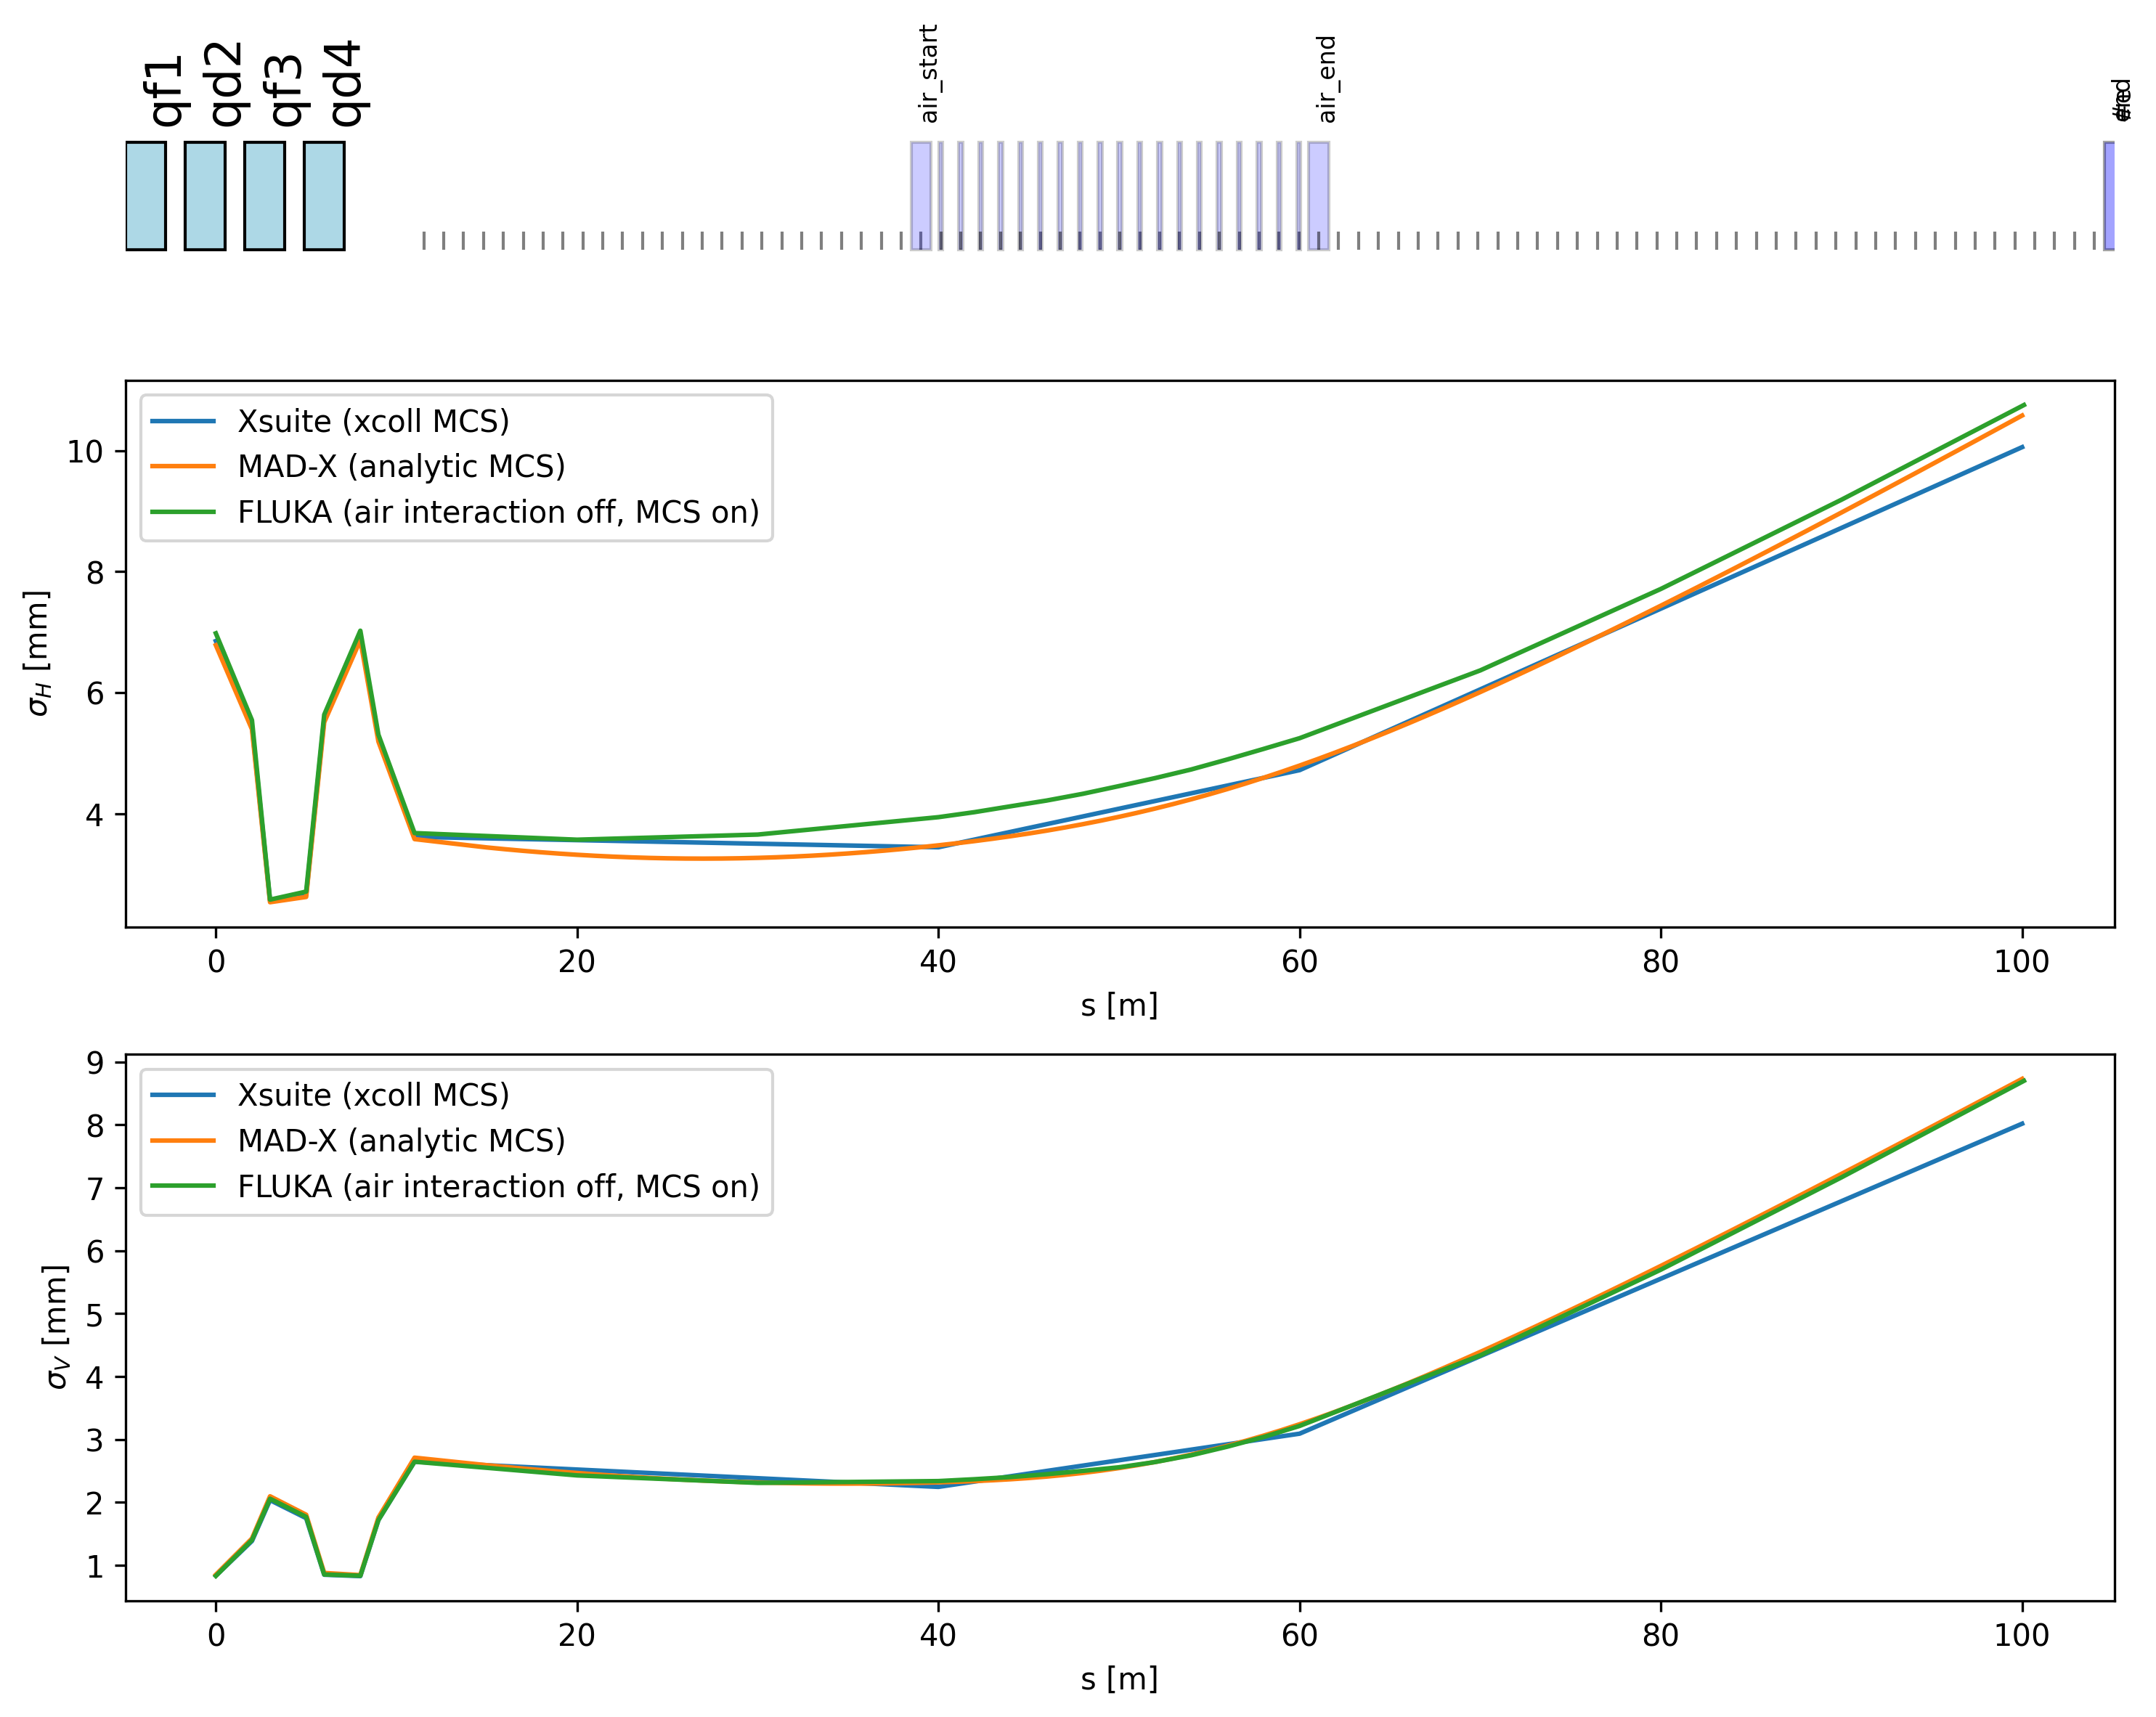
\includegraphics[width=0.7\textwidth]{images/compare_simulation_MCS.png}
\caption{Comparison between Multiple Coulomb Scattering (MCS) models with an air region between 40 and 60 m.}
\label{fig:comparison_sim}
\end{figure}

\newpage
Figure \ref{fig:twiss_param_comparison_with_xsuite} shows a comparison with Xsuite of $\beta_{x,y}$ as well as the emittance blow up. The beta function is almost a perfect match whereas the emittance increase is slightly larger for the MAD-X simulation.

\begin{figure}[!htb]
\centering
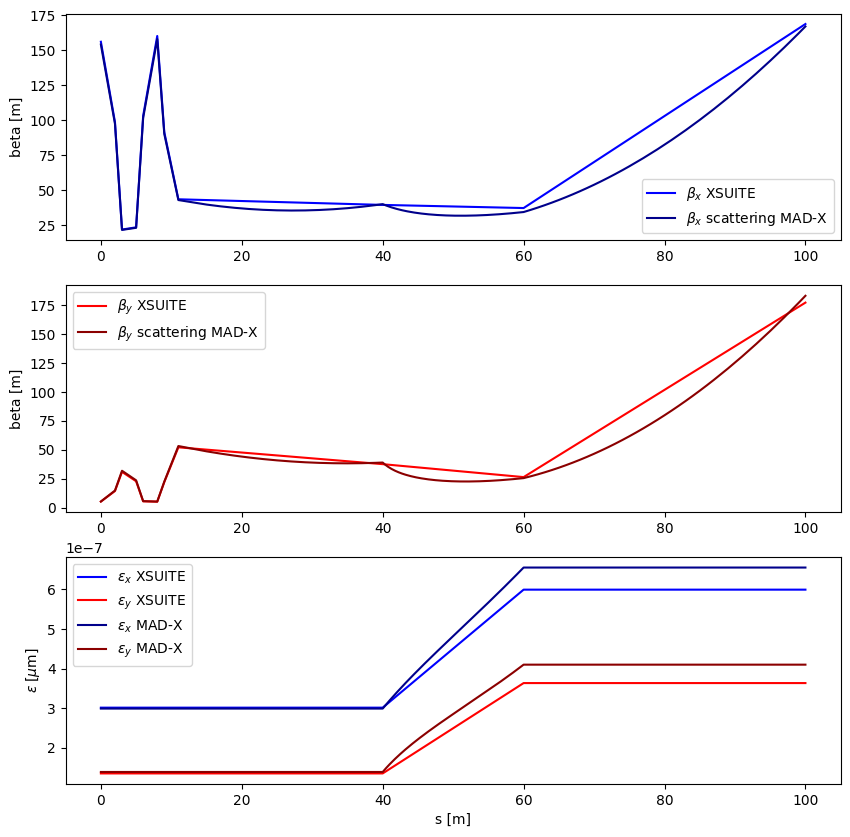
\includegraphics[width=0.8\textwidth]{images/twiss_param_comparison_with_xsuite.png}
\caption{Comparison between MAD-X and Xsuite twiss parameters change and emittance growth.}
\label{fig:twiss_param_comparison_with_xsuite}
\end{figure}

\newpage
\subsection{Tracking PTC}

The analytical measurement was compare to tracking where a distribution of particle are given a random kick (where the kick is sampled randomly from the same $\theta_{RMS}$. For this we use a monte carlo dipole kick. It the same but the speed is much faster.

\begin{figure}[!htb]
\centering
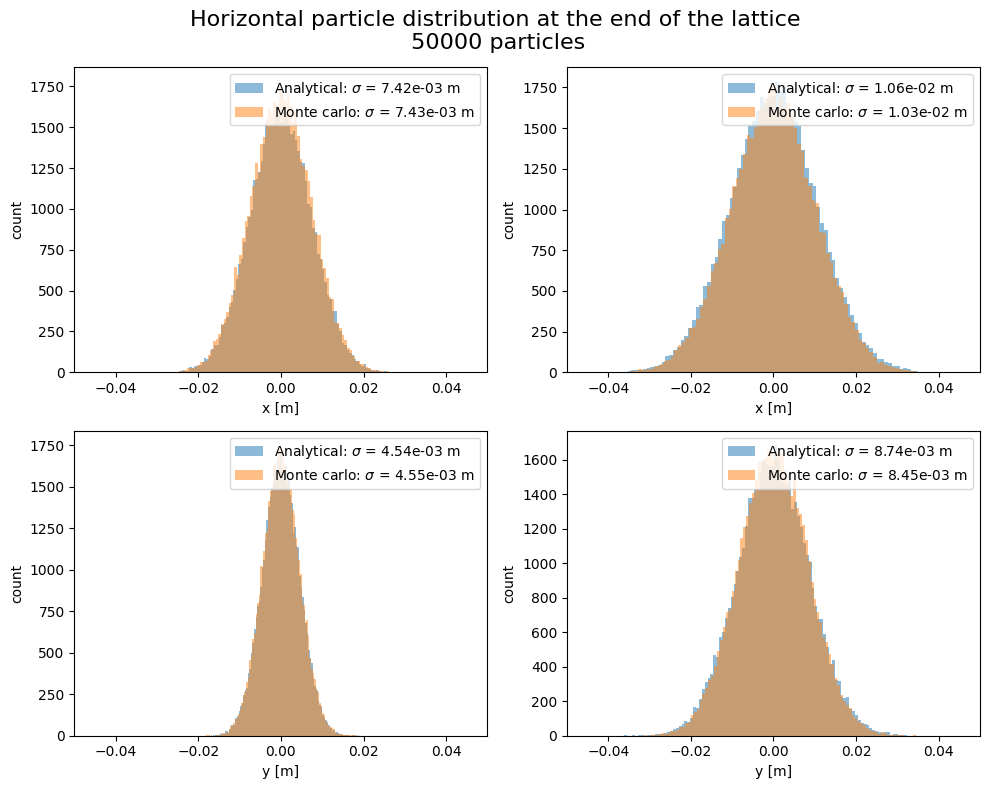
\includegraphics[width=0.8\textwidth]{images/comparison_with_monte_carlo.png}
\caption{Comparison with Monte Carlo.}
\label{fig:comparison_with_monte_carlo}
\end{figure}

\newpage
Table \ref{table:twiss_parameters_table} shows the computed twiss parameters with vacuum and with MCS in both MAD-X analytical and Monte Carlo. This comparison also take the simple $\SI{100}{m}$ line with a $\SI{10}{m}$ air region in the middle. The computation time for 50'000 particles takes around $\SI{30}{minutes}$ with Monte Carlo whereas using the analytical method it takes $\SI{1}{s}$.

\begin{table}[!htb]
\centering
\caption{Twiss parameters at the end of the line}
\label{table:twiss_parameters_table}
\begin{tabularx}{\textwidth}{l*{4}{>{\raggedright\arraybackslash}X}}
\hline
\textbf{Parameter} & \textbf{Analytical Not Scattered} & \textbf{Analytical Scattered} & \textbf{Monte Carlo Not Scattered} & \textbf{Monte Carlo Scattered} \\
\hline
alfx & -2.05 & -2.56 & -2.06 & -2.52 \\
betx & 184.18 & 166.09 & 185.06 & 165.24 \\
ex & 2.98e-07 & 6.58e-07 & 2.98e-07 & 6.38e-07 \\
alfy & -1.71 & -3.19 & -1.71 & -3.13 \\
bety & 149.75 & 182.88 & 149.58 & 179.99 \\
ey & 1.37e-07 & 4.11e-07 & 1.39e-07 & 3.97e-07 \\
\hline
\end{tabularx}
\end{table}


\subsection{Full F61/T08 line}

Figure \ref{fig:full_t08_line_beam_size} shows the full F61/T08 line with and without MCS. The beam size at the end of the line grows from $\SI{6}{}$ to $\SI{8.2}{mm}$ over $\SI{40}{m}$.

\begin{figure}[!htb]
\centering
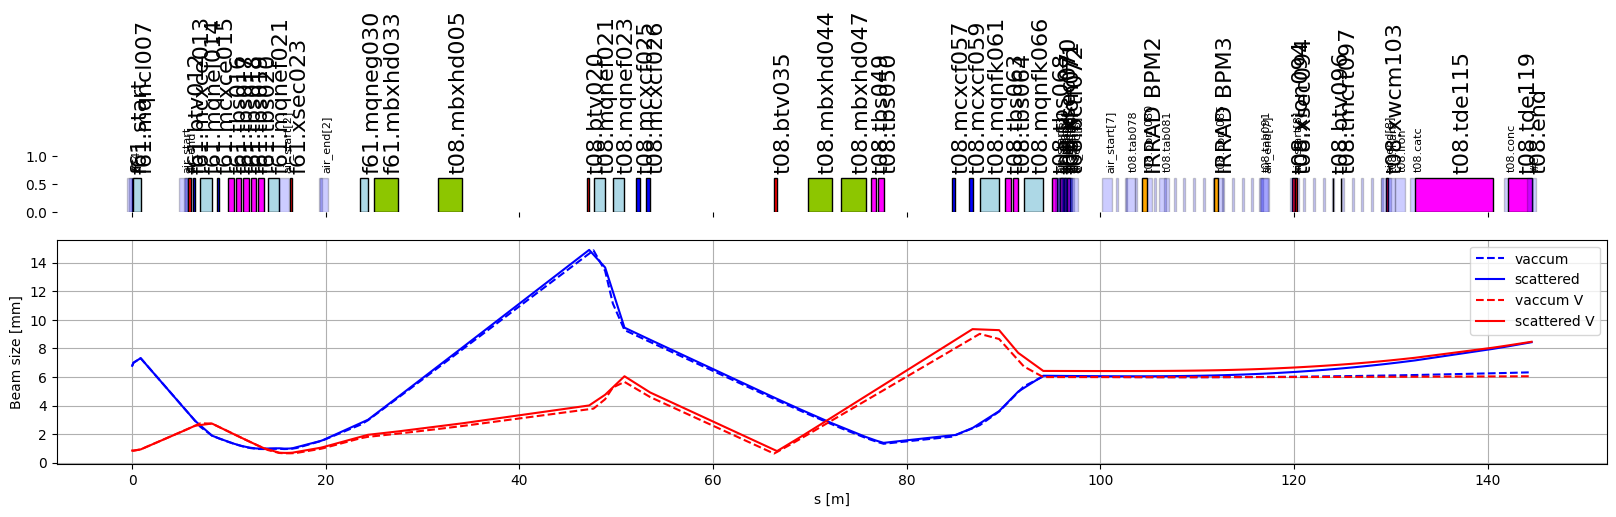
\includegraphics[width=1.0\textwidth]{images/full_t08_line_beam_size.png}
\caption{Full F61/T08 line with and without MCS.}
\label{fig:full_t08_line_beam_size}
\end{figure}

\newpage
\section{Discussion}
% Interpret your results, discuss the implications, and compare with previous work.
% Outline any difficulties encountered during the project.

This simple model only computes MCS which isn't enough to fully describe elastic and inelastic scattering which the FLUKA model can. One observe that multiple coulomb scattering only account for half the increase in beam size whereas the other second half is induced by discrete elastic and inelastic processes that can be modelled in FLUKA. 

\begin{figure}[!htb]
\centering
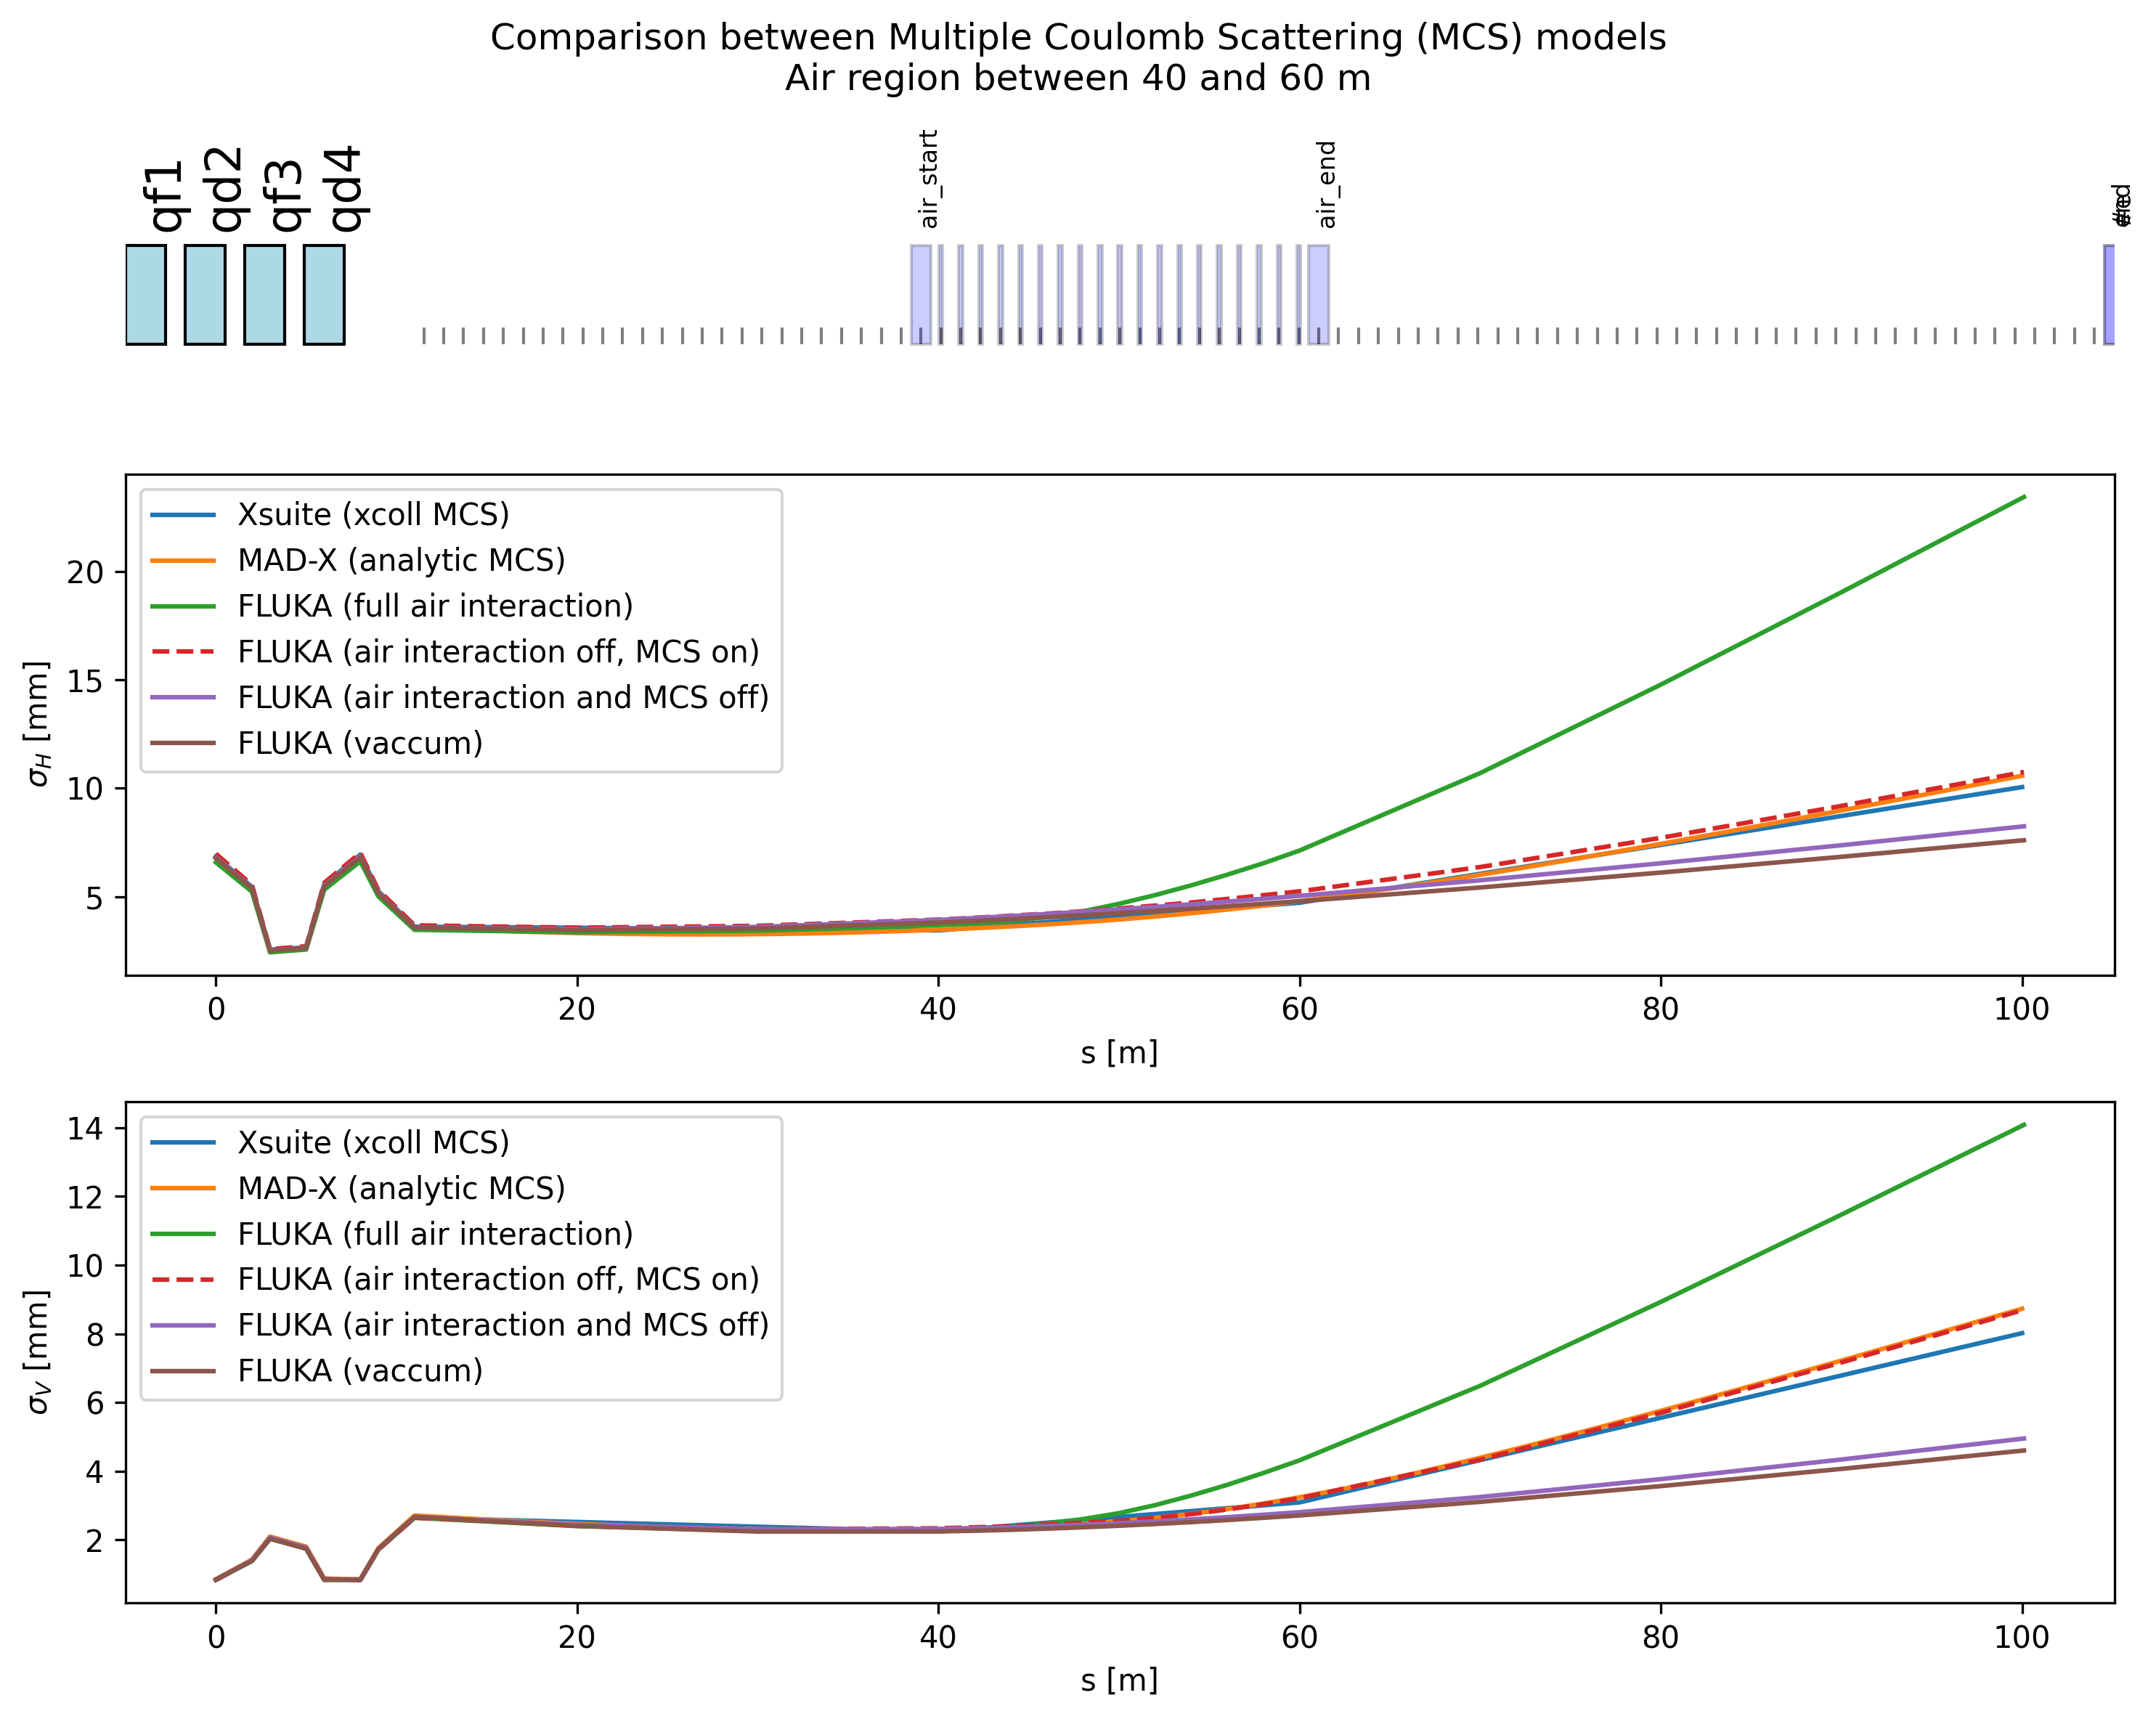
\includegraphics[width=0.8\textwidth]{images/compare_simulation.png}
\caption{Comparison MCS scattering and full air interaction in FLUKA for a $\SI{10}{m}$ air region between $\SI{40}{}$ and $\SI{60}{m}$.}
\label{fig:compare_simulation}
\end{figure}

Another downfall is that energy straggling (i.e. loss in particle momentum) is not computed. This is important for transmission as lower energy beam will have different trajectories if the magnets are not scaled properly. Figure \ref{fig:centroid_displacement} shows the centroid displacement of beam of different energies with respect to the 1 GeV/u beam. This conceives that steering of the beam was done on the high energy beam (which it was) and a linear scaling of the magnets with the PS extracted energy and energy straggling would cause the following centroid displacement. As we can observe, the centroid moves from -1 to +2 cm which could affect transmission if the $\SI{1}{\giga\electronvolt\per\text{u}}$ beam is not perfectly centered. Intersesting to note is the achromat at the end of the line (dispersion = 0) which means that all the beam come back to the same position in CHARM even if the magnets where not properly scaled.

\begin{figure}[!htb]
\centering
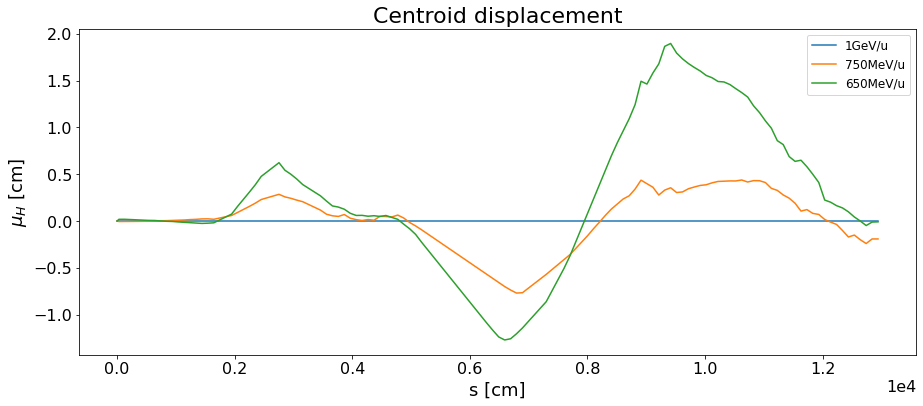
\includegraphics[width=0.8\textwidth]{images/centroid_displacement.png}
\caption{FLUKA calculation of the centroid displacement in the F61/T08 line.}
\label{fig:centroid_displacement}
\end{figure}

Measurement using the IRRAD BPMs show that MCS does not account for the full air scattering beam size blow up the air scattering  and that additional effects need to be taken into account, see Fig. \ref{fig:comparison_to_measurement}.

\begin{figure}[!htb]
\centering
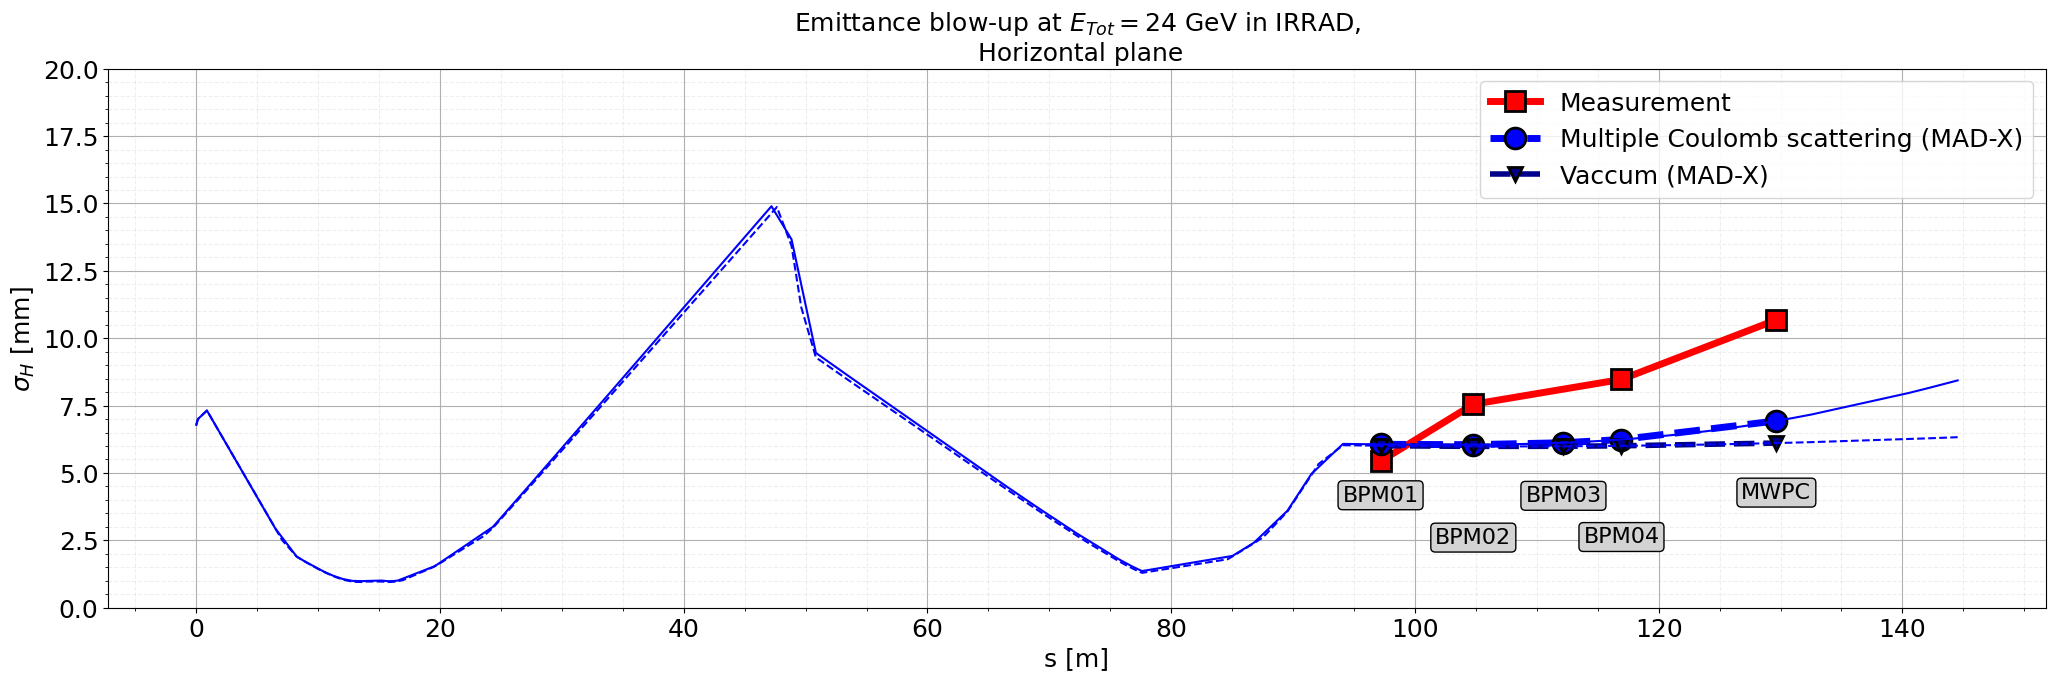
\includegraphics[width=1.0\textwidth]{images/comparison_to_measurement.png}
\caption{Comparison to IRRAD BPM measurement.}
\label{fig:comparison_to_measurement}
\end{figure}


\newpage
\section{Conclusion and Future Work}
% Summarize the impact of your work and propose directions for future research.


\bibliography{references_zotero}
\bibliographystyle{plain}

\end{document}